\documentclass[A4,svgnames,9pt,aspectratio=169]{beamer}
%% document options:
%% - aspectratio = { 43, 169, 1610 }
%% - utf8
%%

%%
%% insert list of packages
%%

%% \usepackage[english,french]{babel}

\hypersetup{ 
   allcolors=bleu_utt_clair,
   pdfauthor   = {firstname lastname},
   pdftitle    = {\@title},
   pdfsubject  = {Resum\'{e} of everything},
   pdfkeywords = {firstname~lastname, curriculum vit\ae{}}
}

%%%%%%%%%%%%%%%%%%%%%%%%%%%%%%%%%%%%%%%%%%%%%%%%%%%%%%%
%%
%%%%%%%%%%%%%%%%%%%%%%%%%%%%%%%%%%%%%%%%%%%%%%%%%%%%%%%
\usepackage{blindtext}
\usepackage{appendixnumberbeamer}

\title[titrecourt]{Template Beamer UTT}
\subtitle{Pour faire des super présentation en utilisant Latek}
\date[00/00/202X]{date long}
\author[A. et al.]{Ducky le canard}
\newcommand{\semester}{A24}
\newcommand{\course}{UE name}


\usetheme{utt}

\begin{document}

% Appeler la page titre
\frame{\titlepage}

% Renommer le titre du sommaire, pour une présentation en anglais par exemple
\renewcommand{\contentsname}{Sommaire}
% Appeler la page de sommaire
%\frame{\tocpage}

%%%%%%%%%%%%%%%%%%%%%%%%%%%%%%%%%%%%%%%%%%%%%%%%%%%%%%%
\section{Utiliser Beamer}
%%%%%%%%%%%%%%%%%%%%%%%%%%%%%%%%% 1ere SLIDE %%%%%%%%%%%%%%
\begin{frame}{Faire sa première slide}
    \begin{block}{exemple d'un "block", élément de base pour beamer}
       Deuxième niveau de liste (Texte courant). Ut wisi enim ad minim veniam, quis nostrud exerci tation
       ullamcorper suscipit loborti. Mauris tempor adipiscing ligula bibendum. Vestibulum sapien lectus,
       porttitor vel euismod a, lobortis at mauris.
   \end{block}

   \begin{block}{2e block}
    Deuxième niveau de liste (Texte courant). Ut wisi enim ad minim veniam, quis nostrud exerci tation
    ullamcorper suscipit loborti. Mauris tempor adipiscing ligula bibendum. Vestibulum sapien lectus,
    porttitor vel euismod a, lobortis at mauris.
\end{block}
\end{frame}

%%%%%%%%%%%%%%%%%%%%%%%%%%%%%%%%% ITEM/ENUMERATE %%%%%%%%%%%%%%
\begin{frame}{List et enumeration}
   \begin{block}{Listes}
      \begin{itemize}
         \item Troisième niveau de liste (Puce 1). Vestibulum sapien lectus, porttitor vel euismod a.
         \begin{itemize}
            \item Quatrième niveau de liste (Puce 2). Netus et malesuada fames ac turpis egestas.
            \item Quatrième niveau de liste (Puce 2). Netus et malesuada fames ac turpis egestas.
            \begin{itemize}
               \item Cinquième niveau de liste (Puce 2). Mauris tempor turpis eu libero sollicitudin.
               \item Cinquième niveau de liste (Puce 2). Mauris tempor turpis eu libero sollicitudin.
            \end{itemize}
          \end{itemize}
        \end{itemize}
   \end{block}

   \begin{block}{Enumerations}
      \begin{enumerate}
         \item Troisième niveau de liste (Puce 1). Vestibulum sapien lectus, porttitor vel euismod a.
         \item Troisième niveau de liste (Puce 1). Vestibulum sapien lectus, porttitor vel euismod a.
         \begin{enumerate}
            \item Quatrième niveau de liste (Puce 2). Netus et malesuada fames ac turpis egestas.
            \item Quatrième niveau de liste (Puce 2). Netus et malesuada fames ac turpis egestas.
            \begin{enumerate}
               \item Cinquième niveau de liste (Puce 2). Mauris tempor turpis eu libero sollicitudin.
            \end{enumerate}
          \end{enumerate}
        \end{enumerate}
   \end{block}
\end{frame}

%%%%%%%%%%%%%%%%%%%%%%%%%%%%%%%%% font size %%%%%%%%%%%%%%
\begin{frame}{Tailles de polices}

   {\tiny         The quick brown fox jumps over the lazy dog}\\
   {\scriptsize   The quick brown fox jumps over the lazy dog}\\
   {\footnotesize The quick brown fox jumps over the lazy dog}\\
   {\small        The quick brown fox jumps over the lazy dog}\\
   {\normalsize   The quick brown fox jumps over the lazy dog}\\
   {\large        The quick brown fox jumps over the lazy dog}\\
   {\Large        The quick brown fox jumps over the lazy dog}\\
   {\LARGE        The quick brown fox jumps over the lazy dog}\\
   {\huge         The quick brown fox jumps over the lazy dog}\\
   {\Huge         The quick brown fox jumps over the lazy dog}

\end{frame}

%%%%%%%%%%%%%%%%%%%%%%%%%%%%%%%%% 2 columns %%%%%%%%%%%%%%
\begin{frame}{Mise en page sur 2 colonnes}
   \begin{columns}
       
       \begin{column}{0.45\textwidth}
            J'en profite pour glisser une equation : 
            \begin{equation}
               \mu_A = \frac{1}{d+1}\sum_{i=1}^{d+1} f(a_i)
            \end{equation}
  
       \end{column}
         
     \begin{column}{0.45\textwidth}
 
            \begin{block}{Premier niveau de liste (Titre)}
            Deuxième niveau de liste (Texte courant).
              \begin{itemize}
                \item Troisième niveau de liste (Puce 1).
                    \begin{itemize}
                      \item Quatrième niveau de liste (Puce 2).
                         \begin{itemize}
                            \item Cinquième niveau de liste (Puce 3).
                         \end{itemize}
                    \end{itemize}
              \end{itemize}
            \end{block}
 
            \begin{block}{Premier niveau de liste (Titre)}
            Deuxième niveau de liste (Texte courant).
              \begin{itemize}
                \item Troisième niveau de liste (Puce 1).
                    \begin{itemize}
                      \item Quatrième niveau de liste (Puce 2).
                    \end{itemize}
              \end{itemize}
            \end{block}
 
          \end{column}
          
   \end{columns}
 \end{frame}


%%%%%%%%%%%%%%%%%%%%%%%%%%%%%%%%%%%%%%%%%%%%%%%%%%%%%%%

%%%%%%%%%%%%%%%%%%%%%%%%%%%%%%%%%%%%%%%%%%%%%%%%%%%%%%%
\section{Elements additionnels}
%%%%%%%%%%%%%%%%%%%%%%%%%%%%%%%%% Blocs %%%%%%%%%%%%%%
\begin{frame}
    \frametitle{Blocks spécifics}
    
    In this slide, some important text will be
    \alert{highlighted} because it's important.
    Please, don't abuse it.
    
    \begin{block}{Simple block}
    Sample text
    \end{block}
    
    \begin{theorem}{Théorème}
    Sample text in red box
    \end{theorem}
    
    \begin{examples}
    Sample text in green box. The title of the block is ``Examples".
    \end{examples}
\end{frame}

%%%%%%%%%%%%%%%%%%%%%%%%%%%%%%%%% Tableaux %%%%%%%%%%%%%%
\begin{frame}
    \frametitle{Tableaux}
    
    \begin{table}[]
        \centering
        \begin{tabular}{|c|c|c|c|}
            \hline
            UE & Semestre & Credits & Responsable  \\
            \hline
             UE 1 & A25 & 18   &  Mr. Tomate  \\
             UE 2 & P24 & 12   &  Mr. Poireau  \\
             UE 3 & A24 & 16   &  Mr. Patate  \\
             \hline
        \end{tabular}
        \caption{Exemple d'un tableau}
        \label{tab:surrogates}
    \end{table}
\end{frame}

%%%%%%%%%%%%%%%%%%%%%%%%%%%%%%%%% FIGURES %%%%%%%%%%%%%%
\begin{frame}{Figures}
    \begin{figure}
        \centering
        
\includegraphics[width=0.3\textwidth]{assets/imgs/img_utt.png}
        \caption{Insertion d'une figure}
    \end{figure}  
\end{frame}
%%%%%%%%%%%%%%%%%%%%%%%%%%%%%%%%%%%%%%%%%%%%%%%%%%%%%%%

%%%%%%%%%%%%%%%%%%%%%%%%%%%%%%%%%%%%%%%%%%%%%%%%%%%%%%%
\section{Animation}
%%%%%%%%%%%%%%%%%%%%%%%%%%%%%%%%% Animation enumerate %%%%%%%%%%%%%%
\begin{frame}{Animation sur une liste (ou énumeration)}
    This is a text in second frame. 
    For the sake of showing an example.
    
    \begin{itemize}
     \item<1-> Text visible from slide 1
     \item<2-> Text visible on slide 2
     \item<3> Text visible on slide 3
     \item<4-> Text visible on slide 4
    \end{itemize}
\end{frame}

%%%%%%%%%%%%%%%%%%%%%%%%%%%%%%%%% Animation frame %%%%%%%%%%%%%%
\begin{frame}{Animation sur un enumerate}
    \begin{columns}
        \begin{column}{0.45\textwidth}

            \onslide<1,3>\begin{block}{1er block}
                Texte du premier block, visible sur la premiere et la troisième slide.
                
            \end{block}
            
        \end{column}
        \begin{column}{0.45\textwidth}
            \onslide<2>\begin{figure}
                \centering
                
\includegraphics[width=0.5\textwidth]{assets/imgs/img_utt.png}
                \caption{Figure visible seulement sur la 2e}
            \end{figure}  
            
        \end{column}
    \end{columns}
\end{frame}
%%%%%%%%%%%%%%%%%%%%%%%%%%%%%%%%%%%%%%%%%%%%%%%%%%%%%%%

%%%%%%%%%%%%%%%%%%%%%%%%%%%%%%%%%%%%%%%%%%%%%%%%%%%%%%%
\section{Tikz}
%%%%%%%%%%%%%%%%%%%%%%%%%%%%%%%%% TIKZ Figure %%%%%%%%%%%%%%

\begin{frame}{ Une simple figure}
\begin{figure}
    \centering
    \begin{tikzpicture}

    \begin{tikzpicture}[scale = 2]

        \draw[] (0,0) -- (1,0) node(a2)[right] {$a_2$};
        \draw[] (1,0) -- (0.8,0.5) node(a3)[above] {$a_3$};
        \draw[] (0.8,0.5) -- (0,0) node(a1)[left] {$a_1$};
        \node [anchor = north] at (0.5, -0.1){simplex $A$};
        
        \draw[->] (1.2, 0.3) -- (2, 0.3);
        
        \draw[] (2,0) -- (3,0) node(a2b)[right] {$a_2$};
        \draw[] (3,0) -- (2.8,0.5) node(a3b)[above] {$a_3$};
        \draw[] (2.8,0.5) -- (2,0) node(a1b)[left] {$a_1$};
        
        \fill[red] (2.7,0) circle (0.03);
        \draw[red, thick] (2.8,0.5) -- (2.7,0) node(ap)[below] {$a^*$};
        
        \fill[blue!30, opacity = 0.5] (2,0) -- (2.7,0) -- (2.8,0.5);
        \fill[orange!30, opacity = 0.5] (3,0) -- (2.7,0) -- (2.8,0.5);
        
        \node[left of = a3b, anchor = west, blue ]{$A_1$};
        \node[above of = a2b, anchor = north, orange ]{$A_2$};
        
            
        \end{tikzpicture}


\end{tikzpicture}
    \caption{première figure}

\end{figure}
    
\end{frame}

%%%%%%%%%%%%%%%%%%%%%%%%%%%%%%%%%Figure animé %%%%%%%%%%%%%%

\begin{frame}{Figure animé}

    \begin{figure}
        \centering
        \begin{tikzpicture}

    \begin{tikzpicture}[scale = 2]

        \draw[] (0,0) -- (1,0) node(a2)[right] {$a_2$};
        \draw[] (1,0) -- (0.8,0.5) node(a3)[above] {$a_3$};
        \draw[] (0.8,0.5) -- (0,0) node(a1)[left] {$a_1$};
        \node [anchor = north] at (0.5, -0.1){simplex $A$};
        
        \onslide<2->{\draw[->] (1.2, 0.3) -- (2, 0.3);
        
        \draw[] (2,0) -- (3,0) node(a2b)[right] {$a_2$};
        \draw[] (3,0) -- (2.8,0.5) node(a3b)[above] {$a_3$};
        \draw[] (2.8,0.5) -- (2,0) node(a1b)[left] {$a_1$};
        
        \fill[red] (2.7,0) circle (0.03);
        \draw[red, thick] (2.8,0.5) -- (2.7,0) node(ap)[below] {$a^*$};
        
        \fill[blue!30, opacity = 0.5] (2,0) -- (2.7,0) -- (2.8,0.5);
        \fill[orange!30, opacity = 0.5] (3,0) -- (2.7,0) -- (2.8,0.5);
        
        \node[left of = a3b, anchor = west, blue ]{$A_1$};
        \node[above of = a2b, anchor = north, orange ]{$A_2$};}
        
            
        \end{tikzpicture}


\end{tikzpicture}
        \caption{Figure animé}
    
    \end{figure}
    
\end{frame}

%%%%%%%%%%%%%%%%%%%%%%%%%%%%%%%%% Plots %%%%%%%%%%%%%%

\begin{frame}{Graphiques}
    \begin{columns}
        \begin{column}{0.45\textwidth}
            \begin{figure}[h]
                \centering
                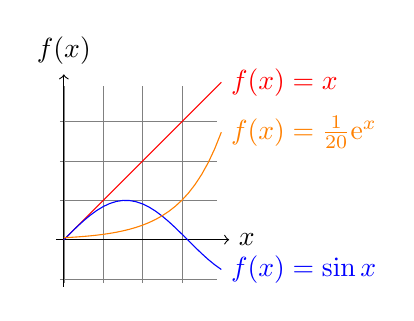
\begin{tikzpicture}[domain=0:4, scale = 0.5]
    \draw[very thin,color=gray] (-0.1,-1.1) grid (3.9,3.9);
  
    \draw[->] (-0.2,0) -- (4.2,0) node[right] {$x$};
    \draw[->] (0,-1.2) -- (0,4.2) node[above] {$f(x)$};
  
    \draw[color=red]    plot (\x,\x)             node[right] {$f(x) =x$};
    % \x r means to convert '\x' from degrees to _r_adians:
    \draw[color=blue]   plot (\x,{sin(\x r)})    node[right] {$f(x) = \sin x$};
    \draw[color=orange] plot (\x,{0.05*exp(\x)}) node[right] {$f(x) = \frac{1}{20} \mathrm e^x$};
\end{tikzpicture}
                \caption{Graphique avec des fonctions}
            \end{figure}
            
        \end{column}
        \begin{column}{0.45\textwidth}
            \begin{figure}[h]
                \centering
                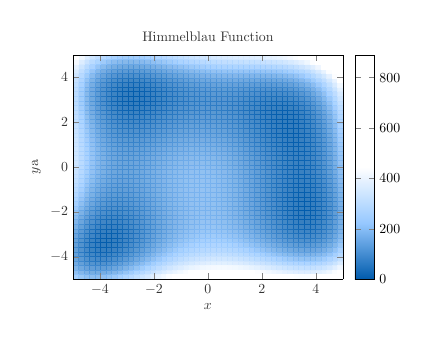
\begin{tikzpicture}[scale = 0.5]
    \begin{axis}[
        colormap={pastel}{ rgb255=(0,91,172) rgb255=(150,200,255) rgb255=(255,255,255)rgb255=(255,255,255)rgb255=(255,255,255)} ,
        view={0}{90},    % Top-down view
        enlargelimits=false,
        axis on top,
        colorbar,        % Add a colorbar
        xlabel=$x$, ylabel=$y$a,
        title={Himmelblau Function},    
        fill opacity=0.8    
    ]
    \addplot3[surf,shader=flat,z buffer=sort,samples=50,domain=-5:5] 
        { (x^2 + y - 11)^2 + (x + y^2 - 7)^2 };
    \end{axis}
\end{tikzpicture}
                \caption{Heatmap pour une fonction prenant 2 dimensions comme argument}
            \end{figure} 
            
        \end{column}
    \end{columns}
\end{frame}


%%%%%%%%%%%%%%%%%%%%%%%%%%%%%%%%%%%%%%%%%%%%%%%%%%%%%%%


%%%%%%%%%%%%%%%%%%%%%%%%%%%%%%%%%%%%%%%%%%%%%%%%%%%%%%% 
\section{Conclusion}
\begin{frame}{Conclusion}
    Une conclusion
\end{frame}


%%%%%%%%%%%%%%%%%%%%%%%%%%%%%%%%%%%%%%%%%%%%%%%%%%%%%%%
\appendix
%% Le texte est modifiable en changeant \thankyou
%% \renewcommand{\thankyou}{Thank You.}
\frame{\merci}


\begin{frame}{Annexes \ref{ap:llm_architecture} : Transformer architecture}
    \label{ap:llm_architecture}
    \begin{figure}
        \centering
        \begin{tikzpicture}[node distance=0.8cm]


    \tikzstyle{norm} = [rectangle, rounded corners, minimum width=1cm ,text centered, draw=black, fill=red!30]
    \tikzstyle{mha} = [rectangle,rounded corners, minimum width=2cm , text centered, draw=black, fill=orange!30]
    \tikzstyle{feed} = [rectangle, rounded corners, minimum width=1cm ,text centered, draw=black, fill=blue!40]
    \tikzstyle{embed} = [rectangle, rounded corners, minimum width=1cm ,text centered, draw=black, fill=pink!30]
    \tikzstyle{encoding} = [rectangle, rounded corners, minimum width=1cm ,text centered, draw=black, fill=pink!40]
    \tikzstyle{linear} = [rectangle, rounded corners, minimum width=1cm ,text centered, draw=black, fill=blue!20]
    \tikzstyle{softmax} = [rectangle, rounded corners, minimum width=1cm ,text centered, draw=black, fill=green!20]
    
    
    \tikzstyle{arrow} = [thick,->,>=stealth]
    \tikzstyle{lightA} = [thick,dotted,->,>=stealth]
    
    \tikzstyle{sum} = [circle, draw, minimum size=0.5cm, node distance=1cm, inner sep=0pt]
    
    % Decoder node
    
    \node (norm3)[norm,yshift = -0.5cm]{Add \& Norm};
    \node (feed2)[feed,below of = norm3, yshift = 0.1cm]{Feed-Forward};
    
    \node (norm4)[norm,below of = feed2,yshift=0.1cm]{Add \& Norm};
    \node (mha2)[mha,below of = norm4, yshift = 0.1cm]{MHA};
    
    \node (norm5)[norm,below of = mha2,yshift=-0.5cm]{Add \& Norm};
    \node (mha3)[mha,below of = norm5]{Masked MHA};
    
    % Encoder node
    
    \node (norm1)[norm,left of = norm4, xshift=-3cm]{Add \& Norm};
    \node (feed1)[feed,below of = norm1]{Feed-Forward};
    
    \node (norm2)[norm,below of = feed1,yshift=-0.5cm]{Add \& Norm};
    \node (mha1)[mha,below of = norm2]{MHA};
    
    % Arrow inside encoder
    \node (enc_base)[below of = mha1]{};
    
    \draw[lightA] (enc_base.center) -- (mha1);
    \draw[lightA] (enc_base.center) -- ([xshift=-0.4cm, yshift = -0.4cm]mha1.south) -- ([xshift=-0.4cm]mha1.south);
    \draw[lightA] ([yshift = -0.3cm]enc_base.center) -- (enc_base.center) -- ([xshift=0.4cm, yshift = -0.4cm]mha1.south) -- ([xshift=0.4cm]mha1.south);
    
    \draw[lightA] ([yshift = -0.3cm]enc_base.center) -- ([yshift = -0.3cm,xshift = -1.3cm]enc_base.center) -- ([xshift = -1.3cm]norm2.center) -- (norm2.west);
    
    \draw [lightA] (mha1) -- (norm2); 
    \draw [lightA] (norm2) -- (feed1); 
    \draw [lightA] (feed1) -- (norm1); 
    
    \draw[lightA] ([yshift = 0.6cm]norm2.center) -- ([xshift = -1.3cm,yshift = 0.6cm]norm2.center) -- ([xshift = -1.3cm]norm1.center) -- (norm1.west);
    
    \node(enc_fit)[draw, thick, dashed, rounded corners, fit=(norm1)(feed1)(norm2)(enc_base), inner sep=0.4cm, label=left:{N $\times$ }] {};
    
    % Arrow inside decoder
    \node (dec_base)[below of = mha3]{};
    
    \draw[lightA] (dec_base.center) -- (mha3);
    \draw[lightA] (dec_base.center) -- ([xshift=-0.4cm, yshift = -0.4cm]mha3.south) -- ([xshift=-0.4cm]mha3.south);
    \draw[lightA] ([yshift = -0.3cm]dec_base.center) -- (dec_base.center) -- ([xshift=0.4cm, yshift = -0.4cm]mha3.south) -- ([xshift=0.4cm]mha3.south);
    
    \draw[lightA] ([yshift = -0.3cm]dec_base.center) -- ([yshift = -0.3cm,xshift = 1.3cm]dec_base.center) -- ([xshift = 1.3cm]norm5.center) -- (norm5.east);
    
    \draw [lightA] (mha3) -- (norm5); 
    
    \draw [lightA] (norm5) --([yshift = 0.4cm]norm5.center) -- ([yshift=-0.4cm,xshift=0.4cm]mha2.south) -- ([xshift=0.4cm]mha2.south); 
    
    \draw [lightA] (mha2) -- (norm4); 
    \draw [lightA] (norm4) -- (feed2); 
    \draw [lightA] (feed2) -- (norm3); 
    
    \draw[lightA] ([yshift = 0.4cm]norm5.center) -- ([xshift = 1.3cm,yshift = 0.4cm]norm5.center) -- ([xshift = 1.3cm]norm4.center) -- (norm4.east);
    \draw[lightA] ([yshift = 0.6cm]norm4.center) -- ([xshift = 1.3cm,yshift = 0.6cm]norm4.center) -- ([xshift = 1.3cm]norm3.center) -- (norm3.east);
    
    \node(dec_fit)[draw, thick, dashed, rounded corners, fit=(norm3)(dec_base), inner sep=0.2cm, label=right:{$\times$ N}] {};
    
    %arrow from encoder to decoder
    
    \draw[arrow] (norm1.north) -- ([yshift=0.4cm]enc_fit.north)
        -- ([yshift=0.4cm, xshift = 2cm]enc_fit.north)
        -- ([yshift=-2.2cm, xshift = 2cm]enc_fit.north)
         -- ([yshift=-2.2cm, xshift = 3.8cm]enc_fit.north)
         -- (mha2.south);
    \draw[arrow] ([yshift = -0.45cm, xshift = -0.4cm]mha2.south) -- ([xshift = -0.4cm]mha2.south);
    
    % encoder input
    \node (enc_plus) [sum, below of = enc_base,yshift=-0.1cm]{\Large $+$};
    \node (in_embed) [embed, below of = enc_plus,align=center, yshift = -0.2cm]{Input \\ Embedding};
    \node (encoding1) [encoding,left of = enc_plus, align = center, xshift = -1.5cm, yshift=-0.2cm]{Positional \\ Encoding};
    \node (input) [below of = in_embed, yshift = -0.3cm]{Input};
    
    % Decoder Input
    \node (dec_plus) [sum, below of = dec_base,yshift=-0.1cm]{\Large $+$};
    \node (out_embed) [embed, below of = dec_plus,align=center, yshift = -0.2cm]{Ouput \\ Embedding};
    \node (encoding2) [encoding,right of = dec_plus, align = center, xshift = 1.5cm, yshift=-0.2cm]{Positional \\ Encoding};
    \node (output) [below of = out_embed, yshift = -0.3cm, align = center]{Ouputs \\ (shifted right)};
    
    %outputs
    \node (linear) [linear, above of = norm3, yshift = -0.1cm]{Linear};
    \node (softmax) [softmax, above of = linear, yshift = -0.1cm]{Softmax};
    \node (out) [above of = softmax,align = center, yshift=-0.1cm]{Output};
    
    
    % I/O arrow
    \draw[arrow] (input) -- (in_embed);
    \draw[arrow] (in_embed) -- (enc_plus);
    
    
    \draw[arrow] (input.west) -- ([ yshift = -0.8cm]encoding1.south) -- (encoding1);
    \draw[arrow] (output.east) -- ([ yshift = -0.8cm]encoding2.south) -- (encoding2);
    
    
    \draw[arrow] (output) -- (out_embed);
    \draw[arrow] (out_embed) -- (dec_plus);
    \draw[arrow] (encoding1) -- (enc_plus);
    \draw[arrow] (encoding2) -- (dec_plus);
    \draw[arrow] (enc_plus) -- ([yshift = -0.3cm]enc_base.center);
    \draw[arrow] (dec_plus) -- ([yshift = -0.3cm]dec_base.center);
    \draw[arrow] (norm3.north) -- (linear);
    \draw[arrow] (linear) -- (softmax);
    \draw[arrow] (softmax) -- (out);
    \draw[arrow] (out.north) -- ([yshift = 0.2cm]out.north);
    
    % Encoder and Decoder Legend
    \node [left of = enc_base,xshift= -2cm, yshift = 1cm]{\textbf{Encoder}};
    \node [right of = dec_base,xshift= 2cm, yshift = 1cm]{\textbf{Decoder}};
    
    \end{tikzpicture}
        \caption{Illustration du mécanisme d'auto-attention : A droite le mécanisme complet, a gauche le \textit{Scaled Dot-product Attention}}
    \end{figure}
    
\end{frame}

\begin{frame}{Annexes \ref{ap:mha} : Multi-Head Attention}
    \label{ap:mha}
    \begin{figure}
        \centering
        \begin{tikzpicture}[node distance=0.8cm]

\tikzstyle{matmul} = [rectangle,rounded corners, minimum width=2cm , text centered, draw=black, fill=purple!30]
\tikzstyle{softmax} = [rectangle,rounded corners, minimum width=2cm , text centered, draw=black, fill=green!30]
\tikzstyle{mask} = [rectangle,rounded corners, minimum width=2cm , text centered, draw=black, fill=pink!30]
\tikzstyle{sca} = [rectangle, rounded corners, minimum width=2cm ,text centered, draw=black, fill=yellow!30]
\tikzstyle{action} = [rectangle, rounded corners, minimum width=2cm ,text centered, draw=black, fill=red!30]
\tikzstyle{arrow} = [thick,->,>=stealth]

\tikzstyle{linear} = [rectangle, rounded corners, minimum width=1cm ,text centered, draw=black, fill=blue!30]
\tikzstyle{dot-prod} = [rectangle, rounded corners, minimum width=2cm,minimum height = 1cm ,text centered, draw=black, fill=purple!50]
\tikzstyle{concat} = [rectangle, rounded corners, minimum width=2cm ,text centered, draw=black, fill=yellow!50]



% Define nodes
\node (matmul1) [matmul]{Matmul};
\node (softmax)[softmax, below of = matmul1, xshift = -0.8cm]{Softmax};
\node (mask) [mask, below of=softmax]{Mask (opt.)};
\node (scale) [sca, below of=mask]{Scale};
\node (matmul2) [matmul, below of=scale]{Matmul};
\node (q) [below of=matmul2, xshift=-0.5cm]{Q};
\node (k) [below of=matmul2, xshift=0.5cm]{K};
\node (v) [below of=matmul2, xshift=1.5cm]{V};


% Draw arrows
\draw [arrow] (matmul1.north) -- ([yshift=0.5cm]matmul1.north);
\draw [arrow] (softmax.north) -- ([xshift=-0.8cm]matmul1.south);
\draw [arrow] (mask.north) -- (softmax.south);
\draw [arrow] (scale.north) -- (mask.south);
\draw [arrow] (matmul2.north) -- (scale.south);
\draw [arrow] (q.north) -- ([xshift=-0.5cm]matmul2.south);
\draw [arrow] (k.north) -- ([xshift=0.5cm]matmul2.south);
\draw [arrow] (v.north) -- ([xshift=0.7cm]matmul1.south);


% MHA 
\node (linear1) [linear, right of = matmul1, xshift = 5cm] {Linear};
\node (concat) [concat, below of = linear1] {Concat};
\node (dot-prod) [dot-prod, below of = concat,yshift= -0.4cm] {Scaled Dot-product Attention};
\node (linear2) [linear, below of = dot-prod, xshift = -1.5cm, yshift = -0.4cm] {Linear};
\node (linear3) [linear, below of = dot-prod, yshift = -0.4cm] {Linear};
\node (linear4) [linear, below of = dot-prod, xshift = 1.5cm, yshift = -0.4cm] {Linear};
\node (q2) [below of=linear2]{Q};
\node (k2) [below of=linear3]{K};
\node (v2) [below of=linear4]{V};

% MHA arrow
\draw [arrow] (q2) -- (linear2);
\draw [arrow] (k2) -- (linear3);
\draw [arrow] (v2) -- (linear4);
\draw [arrow] (linear2.north) -- ([xshift=-1.5cm]dot-prod.south);
\draw [arrow] (linear3.north) -- (dot-prod.south);
\draw [arrow] (linear4.north) -- ([xshift=1.5cm]dot-prod.south);
\draw [arrow] (dot-prod) -- (concat);
\draw [arrow] (concat) -- (linear1);
\draw [arrow] (linear1.north) -- ([yshift=0.5cm]linear1.north);

% MHA * h
\node[draw, thick, dashed, rounded corners, fit=(dot-prod), inner sep=0.1cm, label=right:{$\times$ h}] {};
\node[draw, thick, dashed, rounded corners, fit=(linear2)(linear3)(linear4), inner sep=0.1cm, label=right:{$\times$ h}] {};


% Title
\node (dot_t) [above of = matmul1,yshift=0.5cm] {\textbf{Scaled Dot-Product Attention}};
\node (mha) [above of = linear1,yshift=0.5cm] {\textbf{Multi-Head Attention}};



\end{tikzpicture}
        \caption{Illustration du mécanisme d'auto-attention : A droite le mécanisme complet, a gauche le \textit{Scaled Dot-product Attention}}
    \end{figure}
    
\end{frame}

\begin{frame}{Annexes \ref{ap:lora} : Low Rank Adaptation (LoRA)}
    \label{ap:lora}
    \begin{figure}
        \centering
        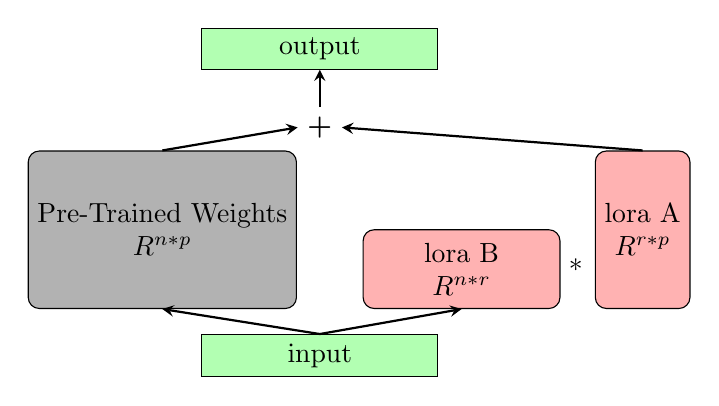
\begin{tikzpicture}[node distance=1.8cm]
    % Define block styles
    \tikzstyle{weights} = [rectangle,rounded corners, minimum width=2.5cm, minimum height=2cm, text centered, draw=black, fill=black!30]
    \tikzstyle{lora_a} = [rectangle,rounded corners, minimum width=1cm, minimum height=2cm, text centered, draw=black, fill=red!30]
    \tikzstyle{lora_b} = [rectangle,rounded corners, minimum width=2.5cm, minimum height=1cm, text centered, draw=black, fill=red!30]
    \tikzstyle{vector} = [rectangle, minimum width=3cm, minimum height=0.5cm, text centered, draw=black, fill=green!30]
    \tikzstyle{arrow} = [thick,->,>=stealth]
    
    % Define nodes
    \node (weights) [weights, align=center]{Pre-Trained Weights \\ $\mathbb{R}^{n*p}$};
    \node (lora_B) [lora_b, right of=weights,xshift=2cm,yshift=-0.5cm, align=center]{lora B\\ $\mathbb{R}^{n*r}$};
    \node (mul) [right of = lora_B,xshift=-0.35cm]{*};
    \node (lora_A) [lora_a, right of=lora_B,xshift=0.5cm,yshift=0.5cm, align=center]{lora A\\$\mathbb{R}^{r*p}$};
    \node (input) [vector,below of = weights, xshift = 2cm,yshift=+0.2cm]{input};
    \node (plus) [above of = weights, xshift = 2cm,yshift=-0.5cm]{\textbf{+}};
    \node (output) [vector,above of = plus,yshift=-0.8cm]{output};
    
    
    
    
    % Draw arrows
    \draw [arrow] (input.north) -- (weights.south);
    \draw [arrow] (input.north) -- (lora_B.south);
    \draw [arrow] (weights.north) -- (plus.west);
    \draw [arrow] (lora_A.north) -- (plus.east);
    \draw [arrow] (plus) -- (output);
    
    
    \end{tikzpicture}
        \caption{Illustration de l'application du Low Rank Adaptation (LoRA)}
    \end{figure}
    
\end{frame}

%%%%%%%%%%%%%%%%%%%%%%%%%%%%%%%%%%%%%%%%%%%%%%%%%%%%%%% 

\end{document}

%%%%%%%%%%%%%%%%%%%%%%%%%%%%%%%%%%%%%%%%%%%%%%%%%%%%%%%
%%
%%%%%%%%%%%%%%%%%%%%%%%%%%%%%%%%%%%%%%%%%%%%%%%%%%%%%%%

